%\documentclass[11pt]{article}

\documentclass[addpoints,10pt]{exam}

\usepackage[margin=2.5cm]{geometry}
\usepackage{graphicx}
\usepackage{listings}
\usepackage{xpatch}
\usepackage{color}
\usepackage{amsmath}

\makeatletter
\xpretocmd{\item@points@pageinfo}{\normalfont}{}{}
\xapptocmd{\item@points@pageinfo}{\bfseries}{}{}
\makeatother

\begin{document}
	\begin{center}
		\LARGE\scshape{Taller 2}
		
		\vspace{1cm}
		\large\scshape{Juan Barbosa - 201325901}
	\end{center}

	\begin{questions}
		{
			\question
			A white floodlight beam crosses a large volume containing a tenuous molecular gas mixture of mostly oxygen and nitrogen. Compare the relative amount of scattering occurring for the yellow (580 nm) component with that of the violet (400 nm) component.
		}
		
		De Rayleigh se sabe que el scattering es proporcional a $1/\lambda^4$:
		\begin{equation}
			S \propto \dfrac{1}{\lambda^4}
		\end{equation}
		
		Entonces el cociente entre el scattering del violeta $(5v)$ y el amarillo $(y)$:
		\begin{equation}
			\dfrac{S_v}{S_y} = \dfrac{1/\lambda_v^4}{1/\lambda_y^4} = \left(\dfrac{\lambda_y}{\lambda_v}\right)^4
		\end{equation}
		\begin{equation}
			S_v = S_y\left(\dfrac{\lambda_y}{\lambda_v}\right)^4 \approx 4.42S_y
		\end{equation}
		
		{
			\question
			A very narrow laserbeam is incident at an angle of 58" on a horizontal mirror. The reflected beam strikes a wall at a spot 5.0 m away from the point of incidence where the beam hit the mirror. How far	horizontally is the wall from that point of incidence?
		}
		
		El \'angulo incidente debe ser igual al reflejado. Lo cual implica que existe un tri\'angulo rect\'angulo con hipotenusa 5.0 m.
		
		\begin{equation}
		\sin(58^\circ) = \dfrac{d}{5.0} \qquad \longrightarrow d = 5\sin(58^\circ) = 4.2\text{ m}
		\end{equation}
		
		{
			\question
			Determine the direction of the exiting ray with respect to the incident ray.
		}
		
		Para la parte superior del espejo, el \'angulo reflejado es igual al incidente. Para el segundo se cumple que est\'a a un \'angulo de 90 $^\circ$, entonces la diferencia es $\theta_r = 90 - \theta_i$.
		
		{
			\question
			Calculate the transmission angle for a ray incident in air at 30$^\circ$ on a block of crown glass (n = 1.52).
		}
		
		Usando la ley de Snell:
		\begin{equation}\label{slope}
			\sin\theta_t = \dfrac{n_i}{n_t}\sin\theta_i
		\end{equation}
		\begin{equation}
			\theta_t = \arcsin\left(\dfrac{n_i}{n_t}\sin\theta_i\right) = \arcsin\left(\dfrac{1.00}{1.52}\sin30\right) = 19.2 ^\circ
		\end{equation}
		
		{
			\question
			Discuss the curve.
			What is the significance of the slope of the line? Guess at what the dense medium might be.
		}
		
		La ecuaci\'on (\ref{slope}) es an\'aloga a la ecuaci\'on de una recta con intercepto $b = 0$. Si $y = \sin \theta_t$ y $x = \sin \theta_i$, la pendiente corresponde con $m = n_i/n_t$. La pendiente se puede calcular como:
		\begin{equation}
			m = \dfrac{y_1 - y_0}{x_1 - x_0} = \dfrac{0.75 - 0.00}{1.00 - 0.00} = \dfrac{0.75}{1.00} = 0.75 \qquad \longrightarrow \qquad n_t = \dfrac{1}{0.75} = 1.33
		\end{equation}
		
		El valor corresponde con el \'indice de refracci\'on del agua.
		
		{
			\question
			Light of wavelength 600 nm in vacuum enters a block of glass where $n = 1.5$. Compute its wavelength in the glass. What color would it appear to someone embedded in the glass?
		}
		
		La definici\'on del \'indice de refracci\'on es:
		\begin{equation}
			n = \dfrac{c}{v} = \dfrac{\nu_0\lambda_0}{\nu_0\lambda'} = \dfrac{\lambda_0}{\lambda'} \qquad \longrightarrow \qquad \lambda' = \dfrac{\lambda_0}{n} = \dfrac{600}{1.5} = \dfrac{2 * 600}{3} = 400 \text{ nm}
		\end{equation}
		
		En la regi\'on de 400 nm, los colores percibidos son azules/violetas.
		
		{
			\question
			An underwater swimmer shines a beam of light up toward the
			surface. It strikes the air-water interface at 35$^\circ$. At what angle will it	emerge into the air?
		}
		
		Usando la ecuaci\'on (\ref{slope}):
		\begin{equation}
			\theta_t = \arcsin\left(\dfrac{n_i}{n_t}\sin\theta_i\right) = \arcsin\left(\dfrac{1.33}{1.00}\sin35\right) = 49.7 ^\circ
		\end{equation}
		{
			\question
			Make a plot of $\theta_i$ versus $\theta_t$, for an air-glass boundary where
			$n_{g} = 1.5$. Discuss the shape of the curve.
		}
		
		\begin{figure}[h]
			\centering
			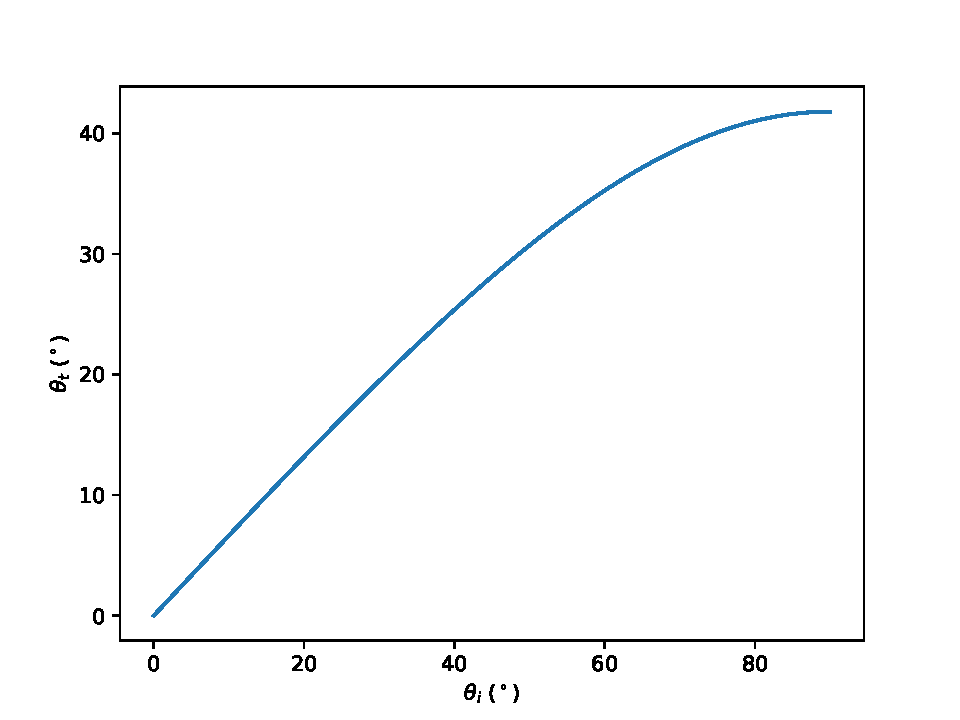
\includegraphics[width = 0.6\linewidth]{418.pdf}
		\end{figure}
		
		{	\question
			A laserbeam having a diameter $D$ in air strikes a piece of glass ($n_{g}$) at an angle $\theta_i$. What is the diameter of the beam in the glass?
		}
		
		La diferencia de camino entre la parte superior del laser y la inferior es $\Delta x$, esta distancia es normal a la direcci\'on del rayo, por lo cual:
		\begin{equation}
			\tan\theta_i = \dfrac{\Delta x}{D} \qquad \longrightarrow \qquad \Delta x = D\tan\theta_i
		\end{equation}
		
		Usando el teorema de Pit\'agoras:
		\begin{equation}
			D'^2 = D^2\tan\theta_i + D^2 = D^2\left(\tan^2\theta_i + 1\right) = D^2\sec^2\theta_i
		\end{equation}
		
		\begin{equation}
			D' = \dfrac{D}{\cos\theta_i}
		\end{equation}
		
		{
			\question
			Calculate the critical angle beyond which there is total internal reflection at an air-glass ($n_g = 1.5$) interface. Compare this result with that of Problem 4.5 (6).
		}
		
		Para la reflexi\'on interna total se calcula el \'angulo incidente para el cu\'al el \'angulo transmitido es 90 $^\circ$.
		\begin{equation}
			\theta_i =  \arcsin\left(\dfrac{n_2}{n_1}\right) = \arcsin\left(\dfrac{1.5}{1.0}\right)
		\end{equation}
		
		Lo anterior no ocurre porque para que exista reflexi\'on interna total, se debe ir de un material \'opticamente m\'as denso a uno menos denso.
		{
			\question
			What is the critical angle for total internal reflection for diamond? What, if anything, does the critical angle have to do with the luster of a well-cut diamond?
		}
		
		Para el diamante el \'indice de refracci\'on es: 2.418, entonces:
		\begin{equation}
			\theta_i = \arcsin\left(\dfrac{1.000}{2.418}\right) = 24.43 ^\circ
		\end{equation}

		{
			\question
			Describe completely the state of polarization of each of the following waves:
			\begin{enumerate}
				\item $\vec{E} = \hat{i} E_0\cos(kz-wt) - \hat{j}E_0\cos(kz - wt)$
				\item $\vec{E} = \hat{i}E_0\sin2\pi(z/\lambda - \nu t) - \hat{j}E_0\sin2\pi(z/\lambda - \nu t)$
				\item $\vec{E} = \hat{i}E_0\sin(\omega t -kz) + \hat{j}E_0\sin(wt-kz-\pi/4)$
				\item $\vec{E} = \hat{i}E_0\cos(\omega t - kz) + \hat{j}E_0\cos(\omega t - kz + \pi/2)$
			\end{enumerate}
		}
		
		La polarizaci\'on puede ser de tres tipos, lineal (un s\'olo plano), circular (dos planos, igual magnitud y desfase de $\pi/2$), y ell\'iptica (dos planos, magnitud distinta o desfase diferente de $\pi/2$).
		\begin{enumerate}
			\item $\vec{E} = (\hat{i} - \hat{j})E_0\cos(kz-wt) \qquad \theta = \arctan(-1) = -45^\circ$ Polarizaci\'on lineal.
			\item $\vec{E} = (\hat{i} - \hat{j})E_0\sin2\pi(z/\lambda - \nu t) \qquad \theta = \arctan(-1) = -45^\circ$ Polarizaci\'on lineal.
			
			\item $\vec{E} = E_0\left(\hat{i}\sin(\alpha) + \hat{j}\sin(\alpha - \pi/4)\right)$ Ambas componentes tienen la misma magnitud, sin embargo existe un desfase de $\pi/4$, esto hace que la polarizaci\'on sea ell\'iptica.
			
			\item $\vec{E} =E_0\left(\hat{i}\cos(\alpha) + \hat{j}\cos(\alpha - \pi/2)\right)$ Ambas componentes tienen la misma magnitud, sin embargo existe un desfase de $\pi/2$, esto hace que la polarizaci\'on sea circular.
		\end{enumerate}
		{
			\question
			A beam of vertically polarized linear light is perpendicularly incident on an ideal linear polarizer. Show that if its transmission axis makes an angle of 60 $^\circ$ with the vertical of only 25 \% of the irradiance will be transmitted by the polarizer.
		}
		
		La ley de Malus:
		\begin{equation}
			I(\theta) = \dfrac{c\epsilon_0}{2}E^1_{01}\cos^2\theta
		\end{equation}
		Para $\theta = 0$ la transmisi\'on de radiaci\'on es total.
		\begin{equation}
			I(0) = I_0 = \dfrac{c\epsilon_0}{2}E^1_{01} \qquad I(\theta) = I_0\cos^2\theta
		\end{equation}
		\begin{equation}
			\dfrac{I(60)}{I_0} = \cos^2 60^\circ = 0.5^2 = 0.25
		\end{equation}
		
		{
			\question
			A glass vessel is placed between a pair of crossed HN-50 linear polarizers, and 50 \% of the natural light incident on the first polarizer is transmitted through the second polarizer. By how much did the sugar solution in the cell rotate the light passed by the first polarizer?
		}
		
		Si no existiera nada en el medio de los polarizadores, dado que ambos son paralelos, se deber\'ia observar intensidad $I = 0$. Sin embargo como la intensidad de salida es igual a la del primer polarizador, la luz debe haber rotado el mismo \'angulo que la diferencia entre los polarizadores, esto es 90$^\circ$.
		
		{
			\question
			Imagine a pair of crossed polarizers with transmission axes vertical and horizontal. The beam emerging from the first polarizer has flux density $I_1$, and of course no light passes through the analyzer ($I_2 = 0$). Now insert a perfect linear polarizer (HN-50) with its transmission axis at 45 $^\circ$ to the vertical between the two elements, compute $I_2$. Think about the motion of the electrons that are radiating in each polarizer.
		}
		
		Las expresiones para cada polarizador son:
		\begin{equation}
			I_1 = I_1
		\end{equation}
		\begin{equation}
			I_m = I_1\cos^2(\theta_m)
		\end{equation}
		\begin{equation}
			I_2 = I_m\cos^2(\theta_2 - \theta_m) =  I_1\cos^2(\theta_m)\cos^2(\theta_2 - \theta_m) = I_1\cos^2(45)\cos^2(45) = I_1\cos^4(45)
		\end{equation}
		
		El resultado es entonces:
		\begin{equation}
			I_2 = I_1\left(\dfrac{\sqrt{2}}{2}\right)^4 = \dfrac{I_1}{4}
		\end{equation}
		
		{
			\question
			Show analytically that a beam entering a planar transparent plate emerges parallel to its initial direction. Derive an expression for the lateral displacement of the beam. Incidentally, the incoming and outgoing rays would be parallel even for a stack of plates of different material.
		}
		
		\begin{figure}[h]
			\centering
			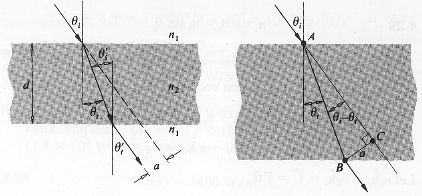
\includegraphics[width = 0.4\linewidth]{demo.png}
		\end{figure}
		
		Por ley de Snell se tiene:
		\begin{equation}
			n_i\sin\theta_i = n_t\sin\theta_t
		\end{equation}
		
		En el lado izquierdo de la figura se observa que los dos rayoz m\'as externos a la izquierda son paralelos, y el superior de ellos tiene \'angulo $\theta_t$, por lo cual $\theta_i' = \theta_t$, de la misma forma se tiene $\theta_i = \theta_t'$.
		
		La distancia entre los puntos $A$ y $B$ (lado derecho) se puede escribir en t\'erminos de el coseno de $\theta_t$.
		
		\begin{equation}
			\cos\theta_t = \dfrac{d}{h} = \dfrac{d}{|B - A|}
		\end{equation}
		
		Usando la misma figura tambi\'en se observa que es posible escribir la distancia como:
		\begin{equation}
			\sin(\theta_i - \theta_t) = \dfrac{a}{h} = \dfrac{a}{|B - A|}
		\end{equation}
		
		Usando las dos ecuaciones anteriores:
		\begin{equation}
			a = \sin(\theta_i - \theta_t)|B - A| = \sin(\theta_i - \theta_t)\dfrac{d}{\cos\theta_t}
		\end{equation}
		
		Como se observa en la figura derecha, $a$ corresponde con el desplazamiento del rayo incidente con el transmitido.
		{
			\question
			Light having a vacuum wavelength of 600 nm, traveling in a glass ($n_g = 1.50$) block, is incident at 45 $^\circ$ on a glass-air interface. It is then totally internally reflected. Determine the distance into the air at which the amplitude of the evanescent wave has dropped to a value of $1/e$ of its maximum value at the interface.
		}
		
		Para una onda electromagn\'etica, para el caso donde $\sin\theta_i > n_{ti}$, donde $n_{ti} = n_{t}/n_{i}$, adem\'as $k_t = 2\pi/\lambda$.
		\begin{equation}
			\beta = k_t\left(\dfrac{\sin^2\theta_i}{n_{ti}^2} - 1\right)^{1/2} = \dfrac{2\pi}{\lambda}\left(\dfrac{\sin^245}{(1/1.5)^2} - 1\right)^{1/2} = \dfrac{2\pi}{600\times10^{-9}}(0.125)^{1/2}= 3702402 \text{ 1/m} \qquad \text{ecuaci\'on 4.72}
		\end{equation}
		
		Tambi\'en se sabe que la amplitud depende de $e^{y\beta}$, por la condici\'on de amplitud, $y\beta = 1$, donde $y$ es la distancia.
		
		\begin{equation}
			y = \dfrac{1}{\beta} = 2.7009\times 10^{-7}\text{ m} = 270 \text{ nm}
		\end{equation}
		
		{
			\question
			Suppose that we look at the source perpendicularly through a stack of $N$ microscope slides. The source seen through even a dozen slides will be noticeably darker. Assuming negligible absorption, show that the total transmittance of the stack is given by:
			\begin{equation*}
				T_t = (1-R)^{2N}
			\end{equation*}
			and evaluate $T_t$ for three slides in air.
		}
		
		Existen dos fronteras en donde hay trasmisi\'on, para cada existe transmisi\'on $T$. Esto implica que para cada placa la transmisi\'on es $T^2$, para $N$ placas, la transmisi\'on total es $T^{2N}$.
			
		La transmisi\'on y la reflexi\'on debe sumar 1.
		\begin{equation}
			T_{total} = T^{2N} = (1-R)^{2N}
		\end{equation}
		
		Para $R$
		\begin{equation}
			R = \left(\dfrac{n_t - n_i}{n_t  + n_i}\right)^2 = \left(\dfrac{1.5 - 1.0}{1.5 + 1.0}\right)^2 = \left(\dfrac{0.5}{2.5}\right)^2 = 0.04
		\end{equation}
		
		La transmisi\'on total para 3 barreras es:
		\begin{equation}
			T_{total} = (1 - R)^(2\times3) = (0.96)^6 = 0.78
		\end{equation}
	\end{questions}
	
	
\end{document}
